\documentclass[12pt, a4paper, oneside]{ctexbook}
\usepackage{amsmath, amsthm, amssymb, bm, graphicx, hyperref, mathrsfs}
\usepackage{geometry}
\usepackage{subfigure}
\usepackage{hyperref}[colorlinks=true,linkcolor=black,citecolor=blue,urlcolor=blue]
\usepackage{pdfpages}

%设置引用格式
\hypersetup{
	colorlinks=true,linkcolor=black,colorlinks=true,linkcolor=black,citecolor=blue,urlcolor=blue
}
%在LateX中,参考文献的引用一般有两种方式,平 齐 时 用 命 令\cite{...}, 上 标 时用\textsuperscript{\cite{...}}

\CTEXsetup[format={\Large\bfseries}]{section}	%section 居左(默认居中)
\CTEXsetup[format={\huge\bfseries}]{chapter}	%chapter 居左(默认居中)


%配置纸张边缘
\geometry{left=2.54cm,right=2.54cm,top=3.18cm,bottom=3.18cm}

\title{{\Huge{\textbf{寄存器说明文档}}}\normalsize{\\——第六届全国大学生集成电路创新创业大赛景嘉微杯初赛提交文档}}
\author{队名:虹ヶ咲学园芯片设计同好会\\ 成员:黄金源\space邓立唯\space林明锋}
\date{\today}
\linespread{1.5}


\begin{document}
	%-----------------------封面------------------
	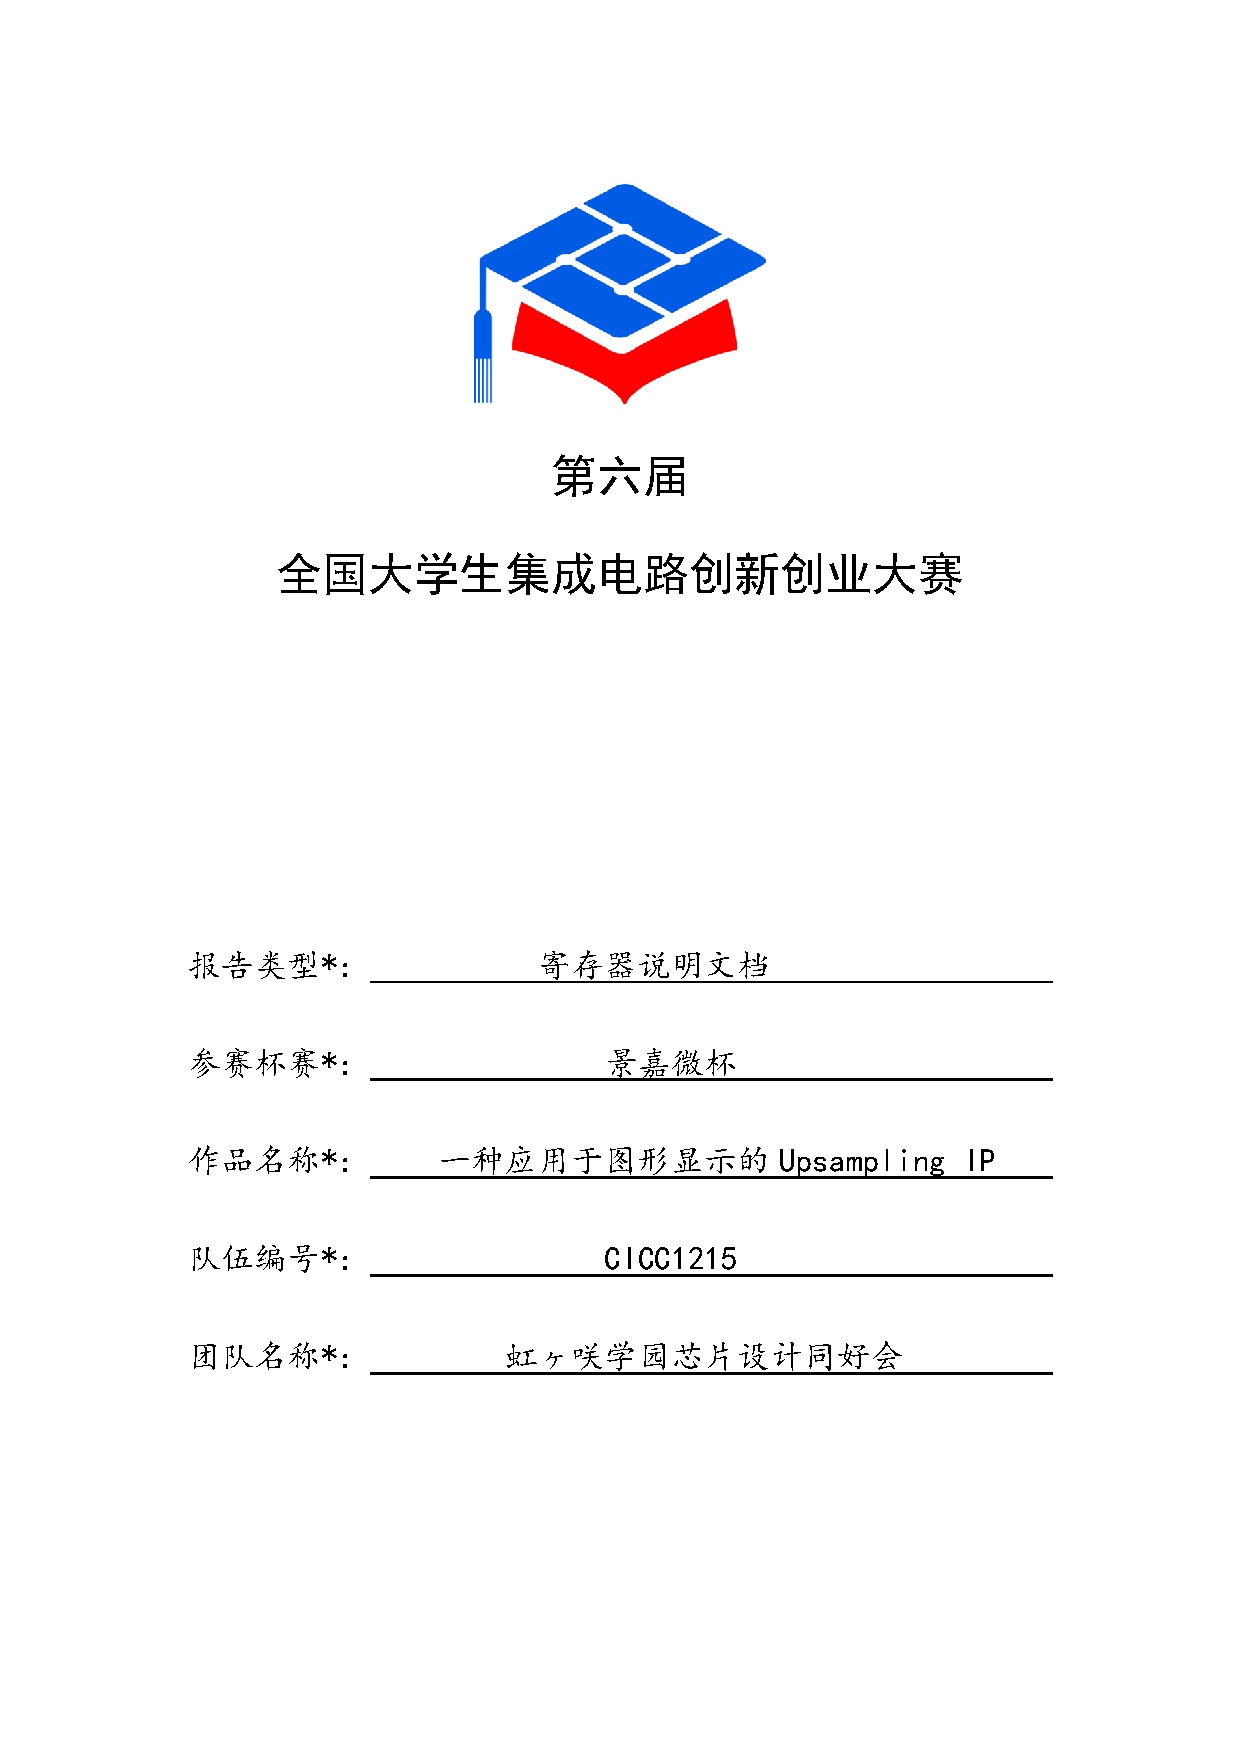
\includepdf{./pic/cover.pdf}
	\maketitle	
	\pagenumbering{Roman}
	\setcounter{page}{1}
	%-----------------------前言------------------
	\begin{center}
		\Huge\textbf{前言}
	\end{center}~\
	
	本文档(寄存器说明文档)仅作为虹ヶ咲学园芯片设计同好会(成员:黄金源、邓立唯、林明锋)参加第六届全国大学生集成电路创新创业大赛景嘉微杯赛初赛提交文档供评委评分使用。
	~\\
	\begin{flushright}
		\begin{tabular}{c}
			虹ヶ咲学园芯片设计同好会\\
			\today
		\end{tabular}
	\end{flushright}
	
	\newpage
	\begin{center}
		{\large 本项目所涉及的 IP 没有使用到寄存器文件进行配置 : )}
	\end{center}


\end{document}